\graphicspath{{./figures}}

\section{Full System}

The South African Weather Service kindly granted permission to track their weather balloons, which have radiosonde payloads. This allowed for full system tests to be conducted, with focus on closed-loop tracking. A first test was conducted near the launch location (Cape Town International Airport), where closed-loop tracking was tested. Although the system computer unfortunately lost power near the 25 km mark, it was observed that the mount correctly steered the antenna based on the received GPS data. The results of both the predicted path and the actual path for this test, as well as the recorded SNR as a function of distance, are shown in Figures \ref{fig:radiosondePredictedVsActual} and \ref{fig:radiosondeSnr}. A second test was conducted from Constantia, around 17 km from launch. The mount correctly pointed towards the launch location using an open-loop uploaded path. Then, at an altitude of $\SI{5.1}{km}$, the system successfully received the radiosonde's GPS location. Unfortunately, due to time constraints, the test was then concluded.

\begin{figure}[!htb]
  \begin{minipage}{.4\textwidth}
    \centering
    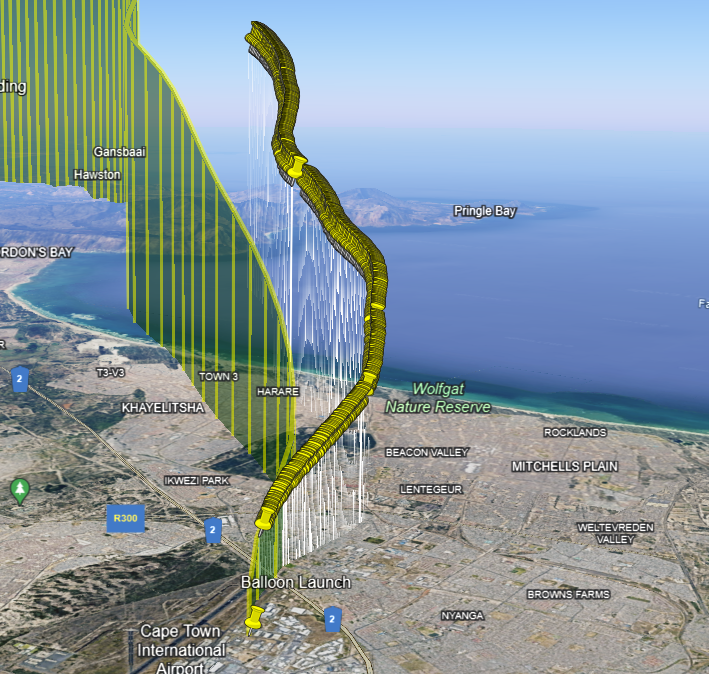
\includegraphics[width=0.98\linewidth]{radiosondePredictedVsActual}
    \caption{Radiosonde Closed-Loop Tracking Predicted Path (left) vs Actual (right)}
    \label{fig:radiosondePredictedVsActual}
  \end{minipage}
  \begin{minipage}{.6\textwidth}
    \centering
    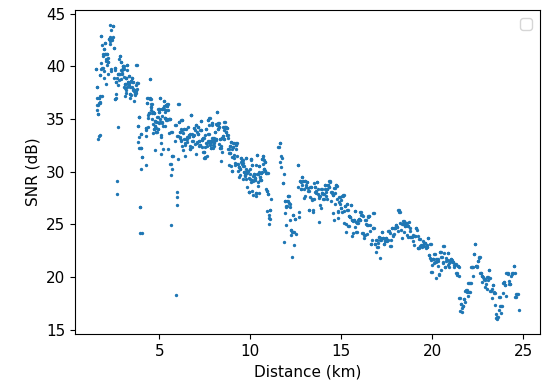
\includegraphics[width=0.98\linewidth]{radiosondeSnr}
    \caption{Radiosonde Closed-Loop Tracking SNR vs Distance}
    \label{fig:radiosondeSnr}
  \end{minipage}
\end{figure}